\documentclass[withoutpreface]{cumcmthesis}
\title{基于logisim的多周期MIPSCPU硬布线控制器设计}

\begin{document}
\maketitle
\begin{tabular}{cccccc}
	\hline
	学  号 & E12214052 &专  业 & 计算机科学与技术 &姓  名 & 赵宸宇 \\
	\hline
	实验日期 & 2024年9月19日 &教师签字 &  &成  绩&\\
	\hline
\end{tabular}
\begin{abstract}
本次实验在上次“多周期微程序mips处理器设计”的基础上复用数据通路,主要完成将\textbf{控制器}的状态控制机制更换为硬布线控制器的设计。同时,作为附加项,学生可以选择是否将控制器的微命令存储器也更换为硬布线逻辑电路。本实验\textbf{的硬布线控制器是纯硬布线的,不包含任何存储设备}。

\subsection*{本次实验的实验产出有:}
\begin{enumerate}
	\item 基于硬布线设计的多周期8指令mipsCPU逻辑电路图:cpu.circ
	\item tex实验报告
	\item 支撑材料(用于状态机相关设计的xlsx表格、py程序等)
	\item 头哥网通关
	\item git日志 请见\url{https://gitee.com/cslearnerer/AHU-CSHT}
\end{enumerate}
\end{abstract}
\tableofcontents
\section{【实验目的】}
实现多周期mipsCPU的\textbf{纯( 可选 | 已选 )}硬布线控制器设计。

完成多周期硬布线mipsCPU整体设计,这包含数据通路设计、控制器设计和程序联调。
\section{【实验原理】}
\subsection{采用硬布线设计以提升性能}
在实验1的基础上,可以通过进一步将微程序控制器升级为硬布线控制器来提升MIPsCPU的运行速度。
\subsection{硬布线控制器和微程序控制器逻辑等价}
\begin{figure}[!h]
	\centering
	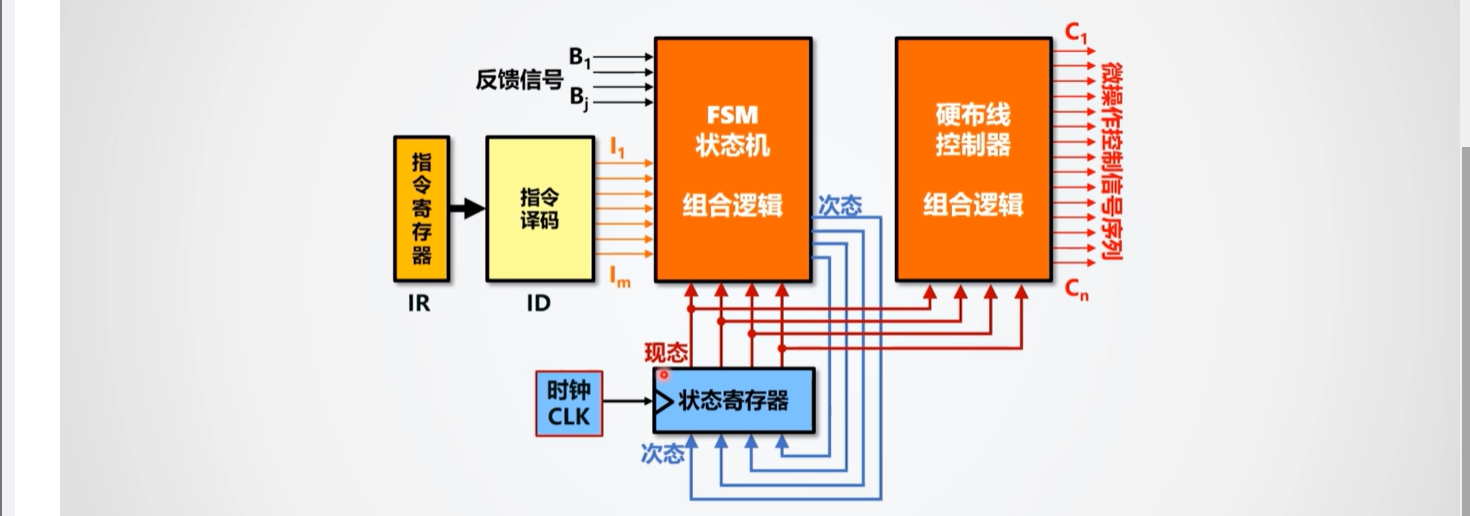
\includegraphics[width=.66\textwidth]{ctrld}
	\caption{控制器顶层设计}
	\label{fig:ctrl-design}
\end{figure}
如\cref{fig:ctrl-design},硬布线控制器由一个状态机和一个组合逻辑电路组成,在功能上和第一次实验中的微程序控制器等价。
\subsection{设计方案}
这里可以实现一个Moore型状态机来提供状态控制,并通过一个组合逻辑电路来读取当前状态输出微命令字段。然后将完成的硬布线控制器嵌入到第一次实验的数据通路中,就完成了CPU电路图的总体设计。
\section{【实验内容】}
\subsection{数据通路的复用}
在本次实验中,我复用了如\cref{fig:reuse}的以下电路:
\begin{figure}[!h]
    \centering
    \begin{minipage}[c]{0.3\textwidth}
        \centering
        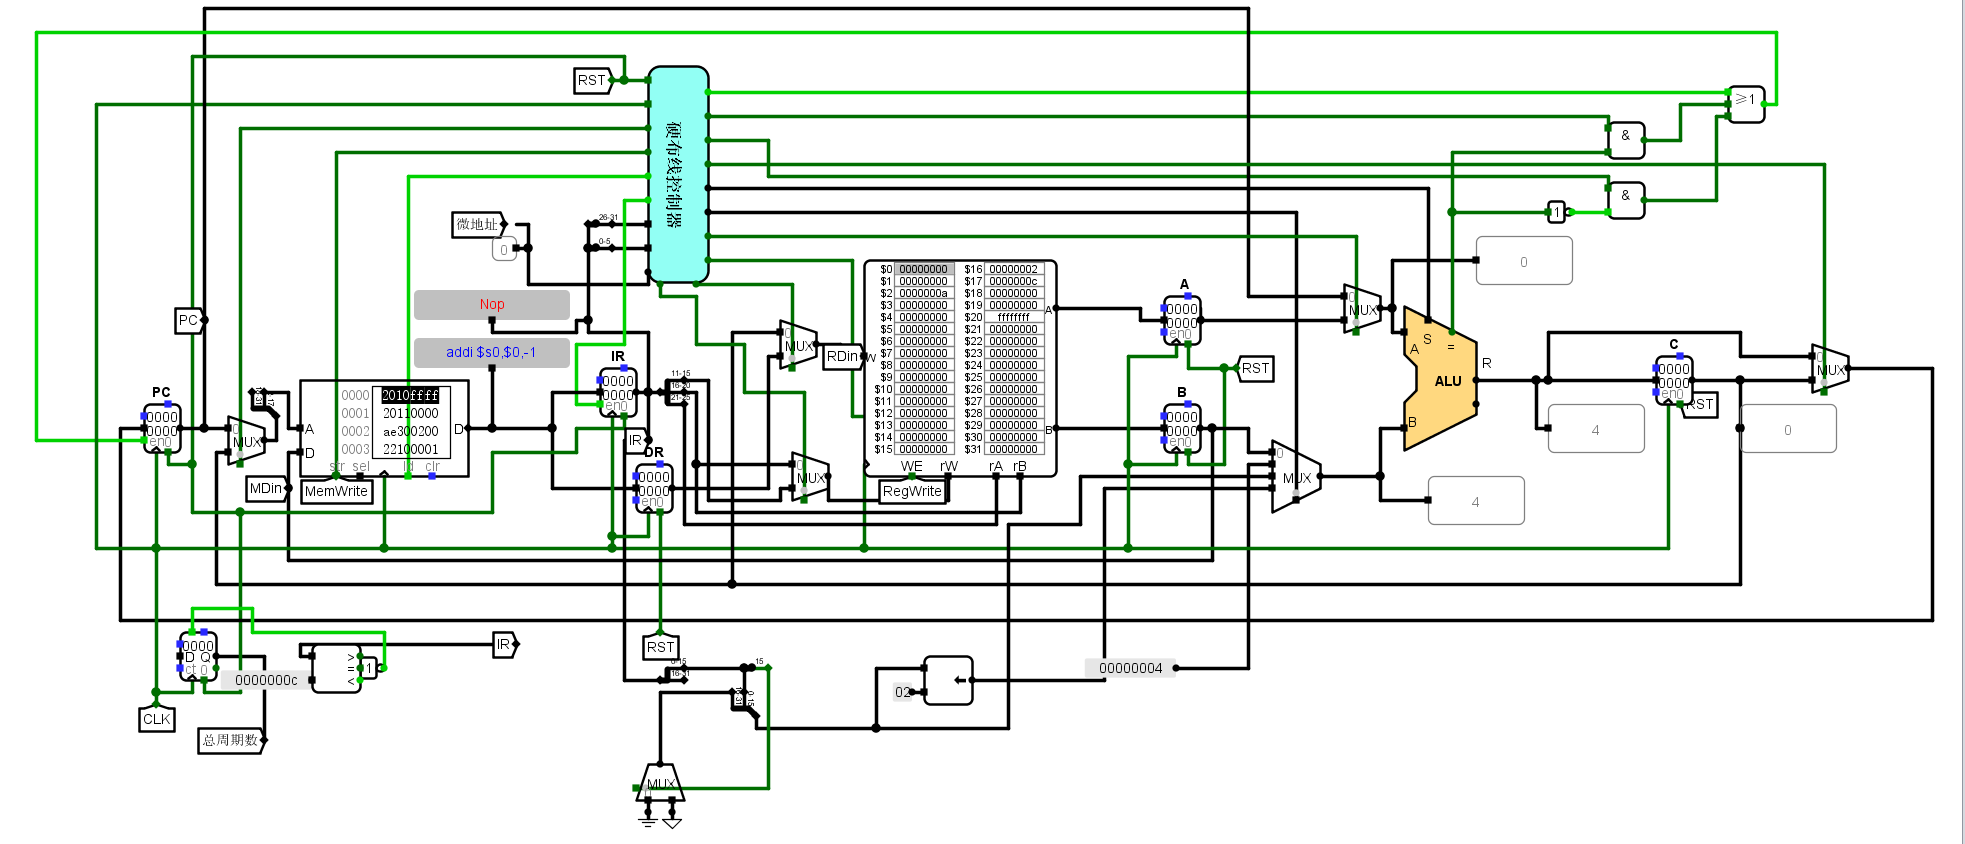
\includegraphics[width=0.95\textwidth]{droad}
        \subcaption{数据通路}
        \label{fig:dr}
    \end{minipage}
    \begin{minipage}[c]{0.3\textwidth}
        \centering
        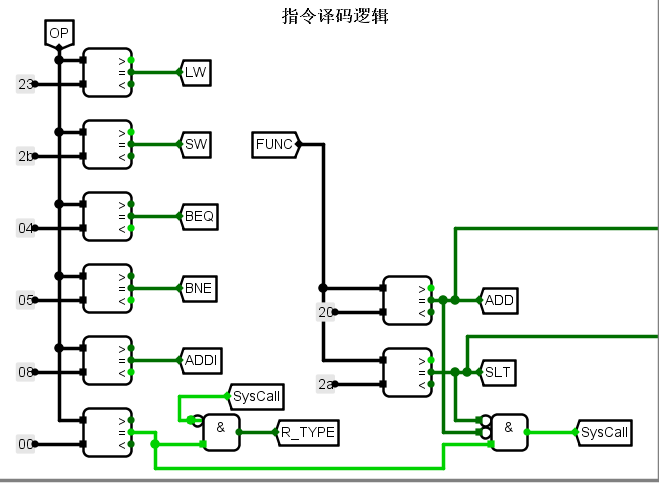
\includegraphics[width=0.95\textwidth]{is}
        \subcaption{指令译码}
        \label{fig:is}
    \end{minipage}
    \begin{minipage}[c]{0.3\textwidth}
        \centering
        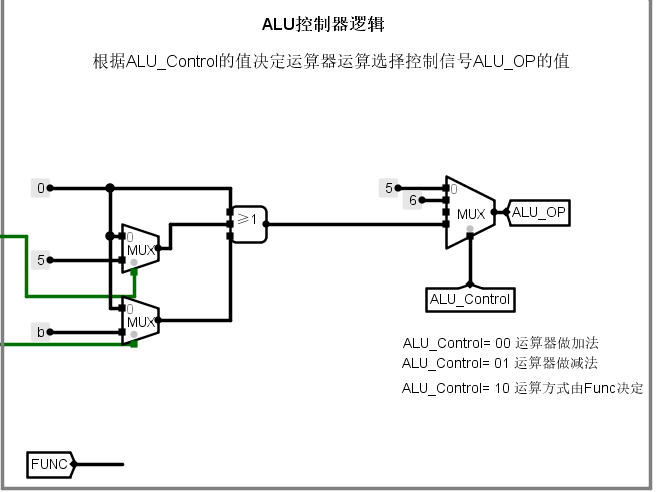
\includegraphics[width=0.95\textwidth]{aluop}
        \subcaption{alu控制}
        \label{fig:aluop}
    \end{minipage}
    \caption{电路复用}
    \label{fig:reuse}
\end{figure}
% check fig posi
\subsection{完成控制器设计}
\begin{figure}[!h]
	\centering
	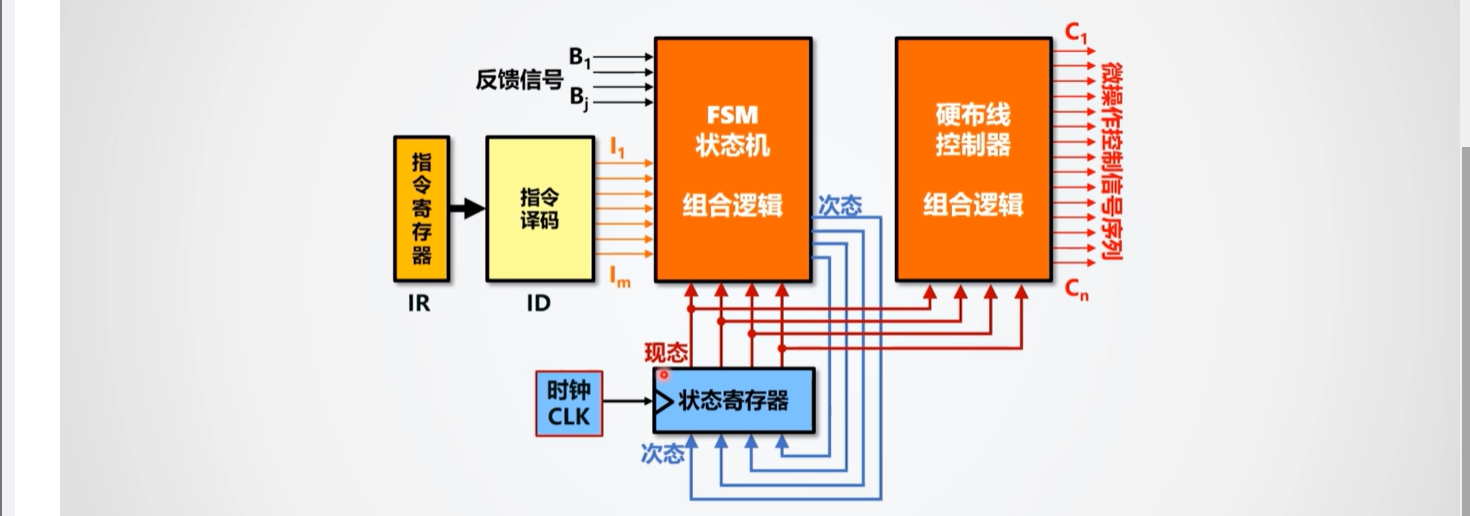
\includegraphics[width=.5\textwidth]{ctrld}
	\caption{控制器顶层设计}
	\label{fig:ctrl-design}
\end{figure}
完成相关电路复用后,首先需要完成控制器状态机的设计。控制器状态机的基本工作原理是接收现态和译码信号、反馈信号,输出多周期指令的下一个工作状态。可以使用xlsx表格,通过刻画状态转移图中的状态转移关系(有向边+条件)来完成FSM状态机这一子电路的组合逻辑设计。结果如\cref{fig:fsm}所示。
\begin{figure}[!h]
\centering
\begin{minipage}[c]{0.2\textwidth}
	\centering
	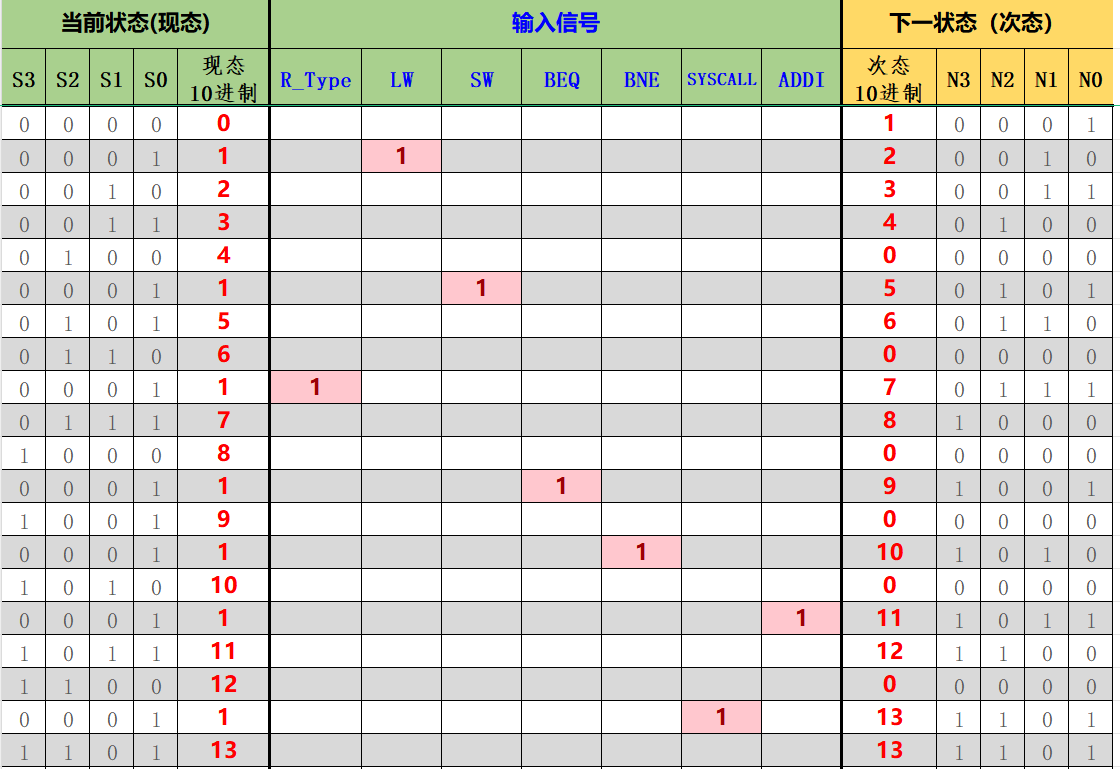
\includegraphics[width=0.95\textwidth]{fsm1}
	\subcaption{状态转移关系}
	\label{fig:fsm1}
\end{minipage}
\begin{minipage}[c]{0.2\textwidth}
	\centering
	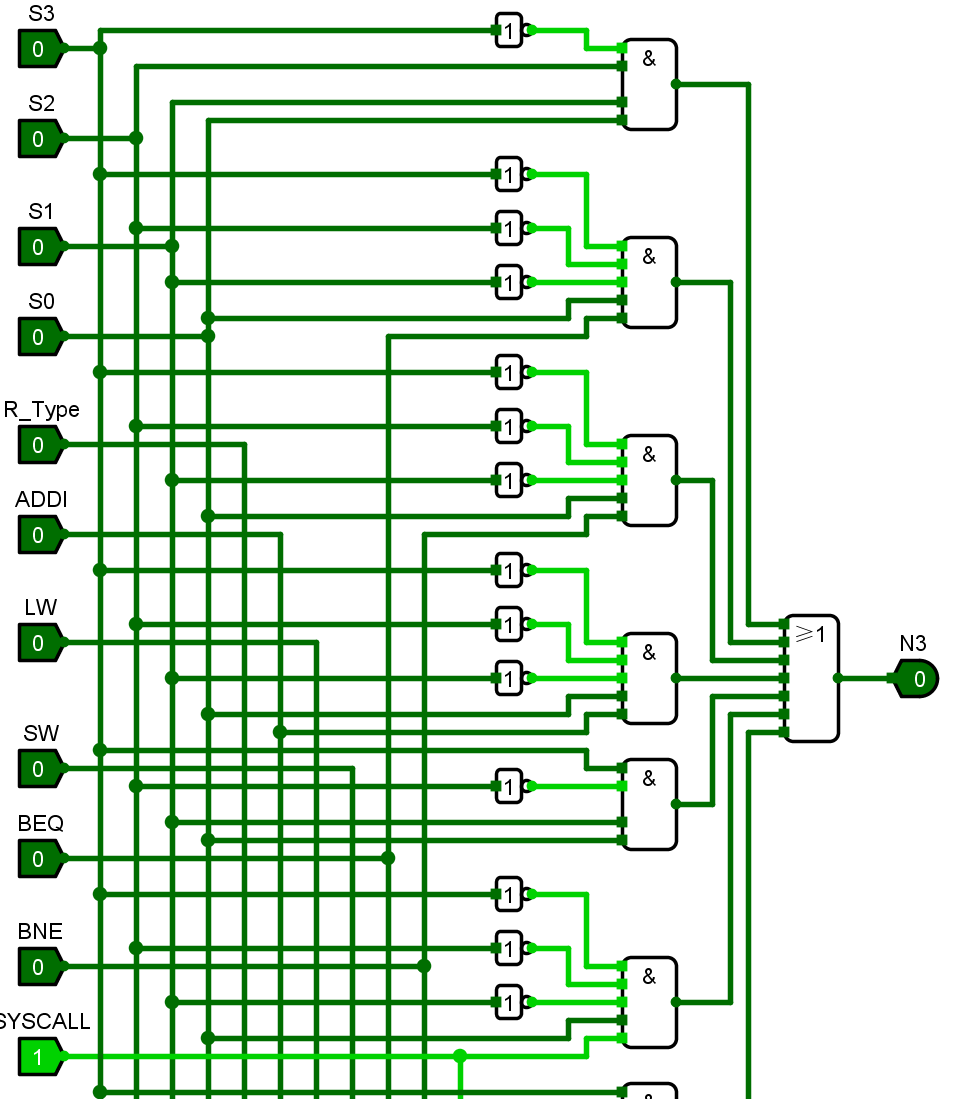
\includegraphics[width=0.95\textwidth]{fsm2}
	\subcaption{电路图}
	\label{fig:fsm2}
\end{minipage}
\caption{FSM状态机}
\label{fig:fsm}
\end{figure}
\subsection{完成硬布线控制器(状态翻译)设计}
对于本次实验设计,可以使用硬布线控制器替代原本的只读存储器。

该硬布线控制器的本质是一个接收4bit输入,给出21bit输出(未优化地址段时)的组合逻辑电路,可以采用如\cref{fig:xlsx-true}的真值表技术配合logisim工程设计功能实现该组合电路的设计。

\begin{figure}[!h]
	\centering
	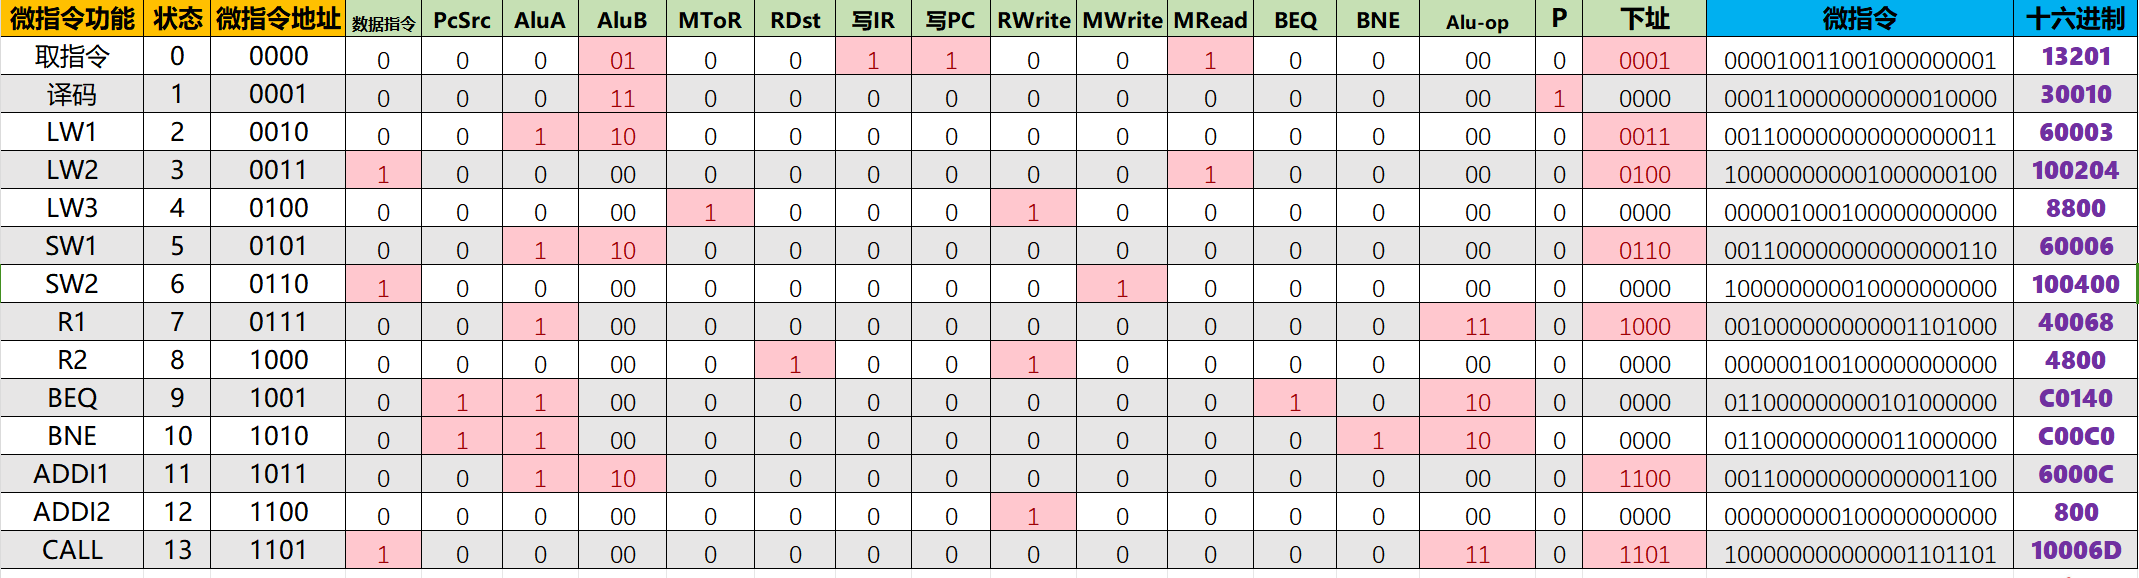
\includegraphics[width=0.66\textwidth]{xlsx-sta}
	\caption{微命令真值表}\label{fig:xlsx-true}
\end{figure}

通过如\cref{fig:design}所示的设计流程,即可得到完全硬布线设计的控制器。

\begin{figure}[!h]
	\centering
	\begin{subfigure}[b]{0.3\textwidth}
		\centering
		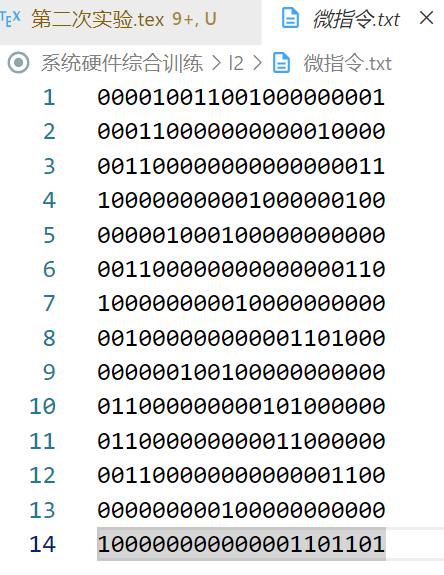
\includegraphics[width=0.95\textwidth]{tiqu}
		\caption{提取真值表}
	\end{subfigure}
	\hfill
	\begin{subfigure}[b]{0.3\textwidth}
		\centering
		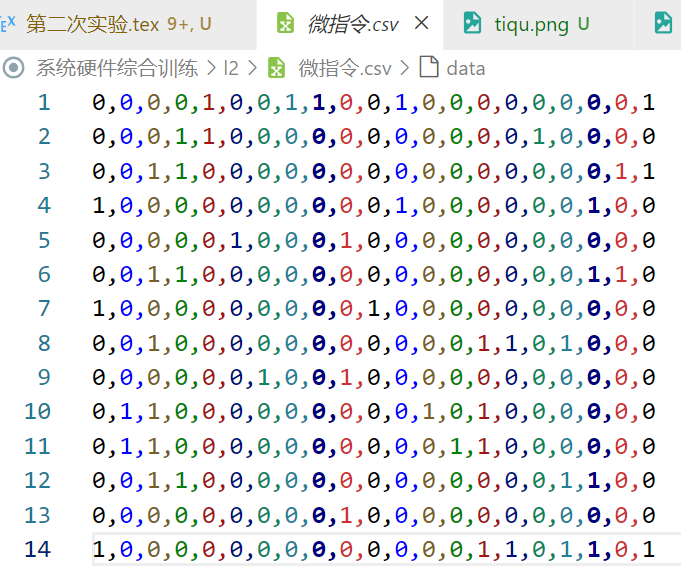
\includegraphics[width=0.95\textwidth]{csv}
		\caption{使用py脚本转换到csv}
	\end{subfigure}
	\hfill
	\begin{subfigure}[b]{0.3\textwidth}
		\centering
		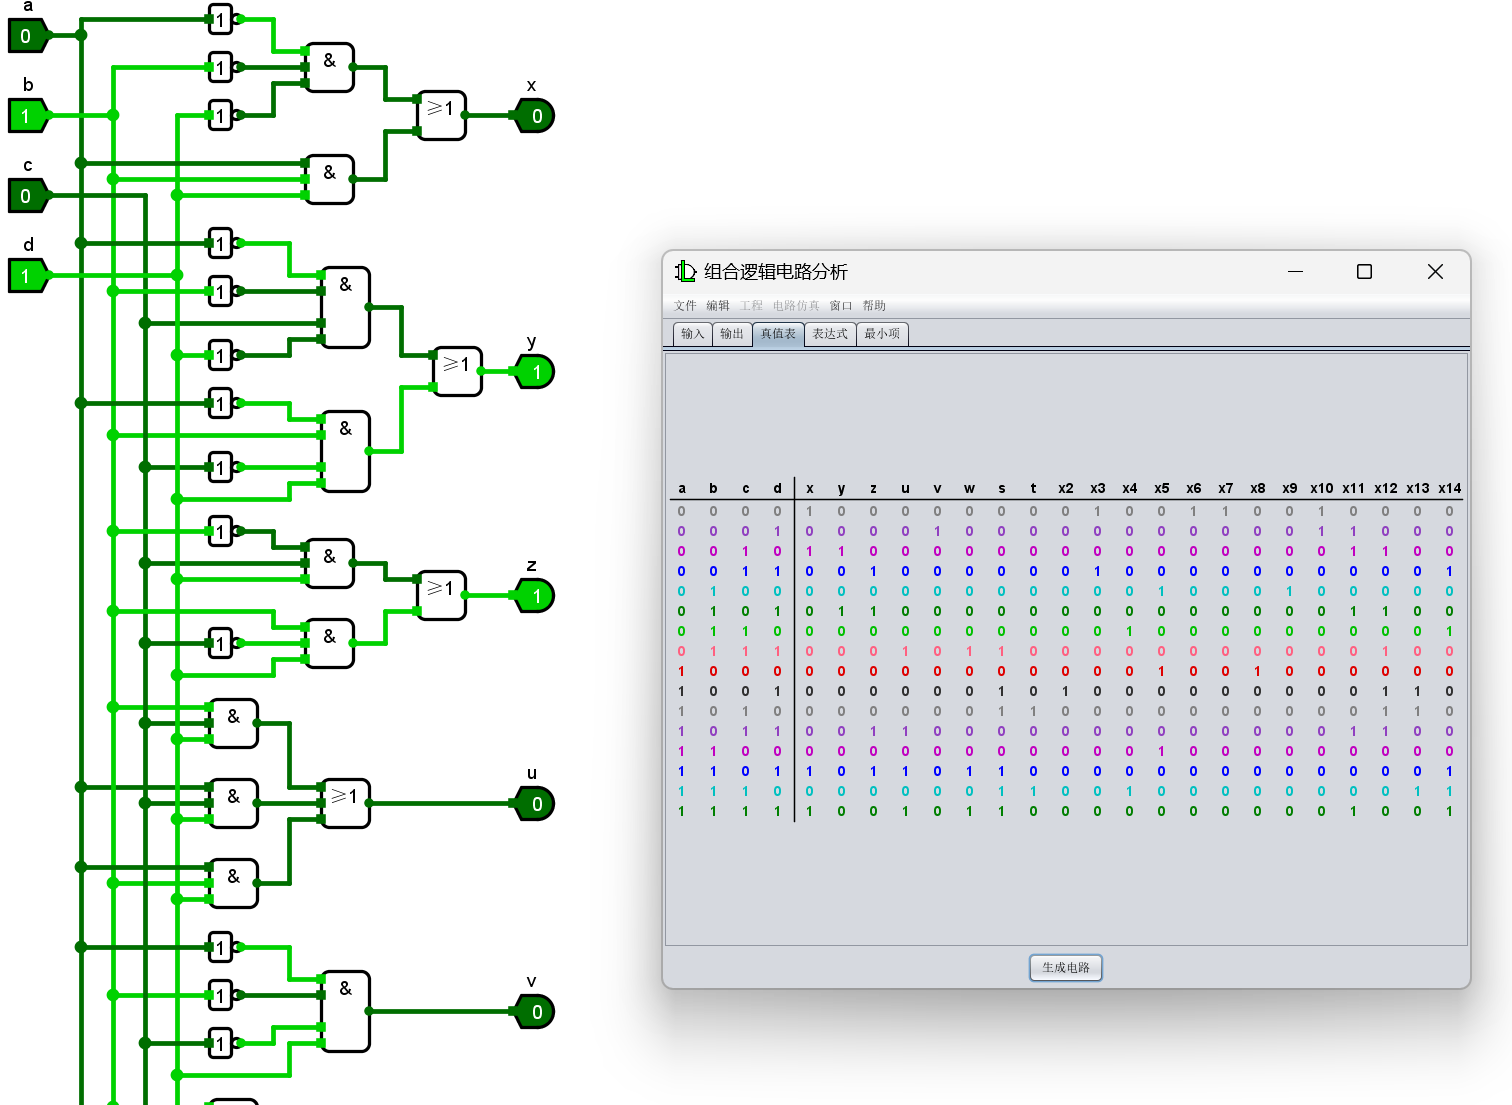
\includegraphics[width=0.95\textwidth]{ic}
		\caption{填写真值表生成电路}
	\end{subfigure}
	\caption{设计流程}\label{fig:design}
\end{figure}

\newpage
\subsection{联调测试}

通过对sort.asm进行测试,经过验证,本次实验直到systemcall指令共运行了891个clk,和标称值891一致。实验测试通过。
\section{【小结讨论】}
在本次实验中,我通过复用相关电路,根据顶层原理独立自主完成了纯硬布线mipsCPU控制器的设计-调试工作。

通过本次实验,我对计算机底层的工作原理理解更深刻,对硬件调试能力得到提升。个人综合工程师素养得到提升。
\subsection{工作展望}
\begin{enumerate}
	\item 优化数据通路图设计,增加可读性和可维护性
	\item 简化微程序字段,这样可以简化硬布线组合逻辑电路,提升CPU性能(提升响应速度,降低发热量,提升$CPI$)。
\end{enumerate}
\end{document}